\documentclass[main.tex]{subfiles} 
\begin{document}

\section*{Teoretisk bakgrunn}

Naturvitenskapen er både et produkt og en prosess. Det vil si på den ene siden er naturvitenskapen en produkt, over en lang historisk utvikling, som er satt sammen av begreper, modeller og teorier som vi idag bruker for å forstå verden rundt oss og prosesser i oss. Ved hjelp av nye oppdagelser og funn utvikler naturvitenskap videre som et produkt. På den andre siden kjennetegnes naturvitenskapen ved sine prosesser og metoder. Naturvitenskapen er ikke bare å vite svar, men å søke nye problemstillinger og sist men ikke minst skape nye erkjennelser  (\citeNP[s.351]{sjob04}). Det er først og fremst denne nysgjerrigheten vi vil skape og kultivere hos våre ungdommer slik at de kan være aktive deltagere i samfunnet. For at dette skal skje er det viktig at undervisningen vektlegger relevans og fremprovoserer nysgjerrighet blant unge mennesker. Videre er det viktig at undervisning tilrettelegges for å oppfylle hver enkelt elevs behov slik at alle elever i en klasse føler at de er deltagende og aktive gjennom undervisningen.

\subsection*{Differensiering}

En av sentrale styringsrammene for norsk utdanningspolitikk og skolepraksis er prinsippet om tilpasset opplæring. Opplæringsloven slår fast at opplæringen skal tilpasses evnene og forutsetningene til den enkelte elev. Opplæringen skal ivareta sentrale verdier som inkludering, variasjon, sammenheng, relevans, verdsetting, medvirkning og erfaringer. Det innebærer at innenfor rammen av ordinære undervisningen, så langt som mulig skal det prøves å tilpasse opplæringen til den enkelte elev. Dette skal operasjonaliseres av undervisere gjennom differensiering (\citeNP[s. 423]{foss14}) og individualisering (\citeNP[s. 129]{tang08}), gjennom blant annet nivå-, mengde- og/eller tempodifferensiering. Undervisningen må derfor tilfredsstille alle elevenes tilretteleggingsbehov i klassen, fra elever med vansker i faget til høytpresterende elever. En viktig intensjon for opplæringsreformen, Kunnskapsløftet (LK06), var nemlig å gi bedre tilpasset opplæring og å styrke elevenes grunnleggende ferdigheter (\citeNP[s. 135]{tang08}; \citeNP[s. 427]{foss14}), som inkluderer blant annet å kunne lese.\footnote{Å kunne lese i naturfag er å forstå og bruke naturfaglige begreper, symboler og figurer. Dette innebærer å kunne identifisere, tolke og bruke informasjon fra lærebøker og digitale kilder (\citeNP{udirLP}).}
\newline\newline
En av vanskelighetene som ligger i gjennomføring av differensiert undervisning er de praktiske forholdene som differensiering og tilpasset opplæring skal gjennomføres i. Blant rammefaktorene som er lagt til rette for at tilpasset undervisning lar seg realisere er et læringsmiljø som er godt utstyrt, både med læringsmateriell og muligheter til å samarbeide og danne grupper (\citeNP[s. 161]{engh11}). I tillegg må læreren ha tilstrekkelig kompetanse til å kunne organisere undervisningen  slik at elever får de faglige utfordringene som er tilpasset deres forutsetninger.
\newline\newline
Ifølge Fosse kan differensiert undervisning deles i to kategorier: \emph{pedagogisk differensiert undervisning} og \emph{organisatorisk differensiert undervisning}. \underline{Permanent} nivådelt undervisning strider mot det overordnede prinsippet tilpasset opplæring (\citeNP[s. 423]{foss14}):
\begin{displayquote}
\textelp{} Til vanlig skal organisering ikke skje etter faglig nivå, kjønn eller etnisk tilhørlighet. (Opplæringsloven)
\end{displayquote}
Fosse referer til metastudie (\citeNP{hatt09}) når hun skriver at de flinke elevene kan dra nytte av organisatorisk differensiert undervisning, men det har ikke ønsket effekt for elever som strever med faget (\citeNP[s. 423]{foss14}).


\subsection*{Motivasjon}

I min praksisperiode har jeg hatt elever som har hatt problemer med motivasjon. Dette har ofte resultert i at deres innsats og utbytte i timen har vært ``minimalistisk''. Smith fremhever at først må elevens vilje være til stede før det kan jobbes med elevens motivasjon (\citeNP[s. 26]{smit09}). Dermed må det arbeides med å styrke elevens tro på seg selv før presset blir lagt på det faglige innholdet. Klarer læreren å skape individuell faglig interesse hos eleven 
\begin{displayquote}
\textelp{} vil en stor del av læringsprosessen bli styrt av eleven selv. Lærerens rolle blir da hovedsakelig å stake ut veien for elevens læring, og det er mindre behov for at læreren må passe på at eleven arbeider med sin egen læring. \newline (\citeNP[s. 26]{smit09})
\end{displayquote} 
Motivasjon blir ofte kategorisert som indre og ytre motivasjon (\citeNP[s. 162]{mang13}; \citeNP[s. 26 - 27]{smit09}). Frøyland lister opp følgende komponenter for å skape indre motivasjon blant elever (\citeNP[s. 36 - 37]{froy10}). Ifølge henne dannes indre motivasjon hos eleven når, eleven:
\begin{itemize}
\item konstruerer personlig mening, 
\item opplever valgfrihet,
\item opplever det utfordrende,
\item opplever at de har kontroll,
\item samarbeider om oppgaver,
\item opplærer at læring har konsekvenser.
\end{itemize}
Forholdet mellom elev og lærer har et vesentlig bidrag til elevenes resultater og skolefaglige interesser (\citeNP[s. 70]{hobo11}). En god relasjon mellom lærer og elev avhenger i hvilken grad elevene føler at de blir forstått og lyttet til. Det er samt viktig å skape situasjoner der elever kan vise mestring. Lav faglig selvtillit kan i en del tilfeller være et reelt hinder for at elever senere velger realfag i videregående utdanning, spesielt blant jenter (\citeNP[s. 225]{abhk11}).

\subsection*{Kompetansemål}

Gjennom noen av mine samtaler med elever i praksisperioden, oppdaget jeg fort at det var få som trakk forbindelsen mellom egen læring og koblingen til kompetansemålene. For undervisere regnes det som en god praksis at elevene er alltid bevisste om hvorfor de lærer det de lærer og hvor de er på vei. \citeA[s. 136]{klet13} beskriver en god undervisningsseksens der lærere klarer å balansere mellom tilegnelses-, utprøvings-, og konsolideringssituasjoner. Ifølge Klette har norske klasserom ensidige tendenser i bruken av varierte arbeidsmåter. Slik det kan ses fra figur \ref{fig:odeg10}, er det for eksempel lite konsolideringssituasjoner. Lærernes metalæringsaktiviteter regnes som særlig avgjørende for å sikre elevenes læring (\citeNP[s. 186]{klet13}). Å bruke dette som et fast organiserende prinsipp, blir derimot sjelden gjennomført (\citeNP[s. 26]{odeg10}). Dermed er det viktig å koble inn kompetansemålene og jobbe målrettet mot høyere kompetansenivå. Dette vil fremme læing hos eleven og gi eleven en pekepinn på hvor hen må ta tak. \newline

\begin{figure}[h!]
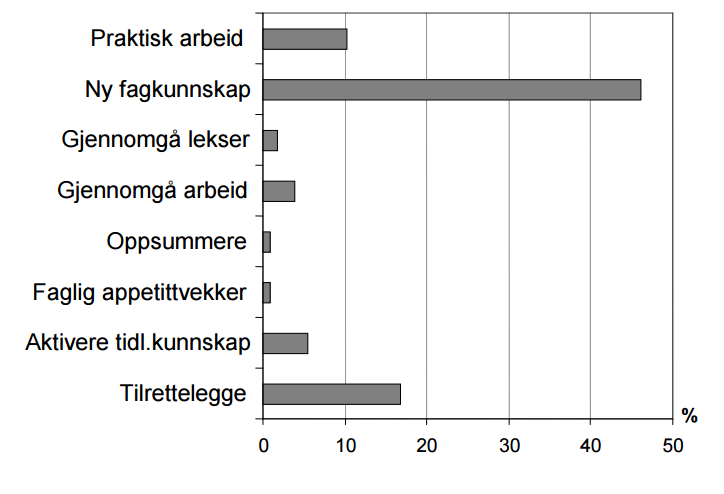
\includegraphics[scale = 0.6]{../figures/undervisnings_aktivitet.png}
\caption{Oversikt over naturfaglærernes undervisningstilbud til elevene fra PISA+ studie. Kilde: 
\protect\citeA{odeg10}.}
\label{fig:odeg10}
\end{figure}

\subsection*{Gruppearbeid}

Et funn innenfor utdanningsforskning er at hjemmebakgrunn har sterk sammenheng med elevers faglig prestasjoner (\citeNP[s. 176]{berg16}). Et viktig mål for norsk skole er å utjevne sosiale forskjeller mellom elevene. Bergem fremhever faktoren som styrker elevenes hjemmebakgrunn og deres prestasjoner, er hovedsakelig lekser. Hans undersøkelse viste at jo flere lekser som gis, \emph{jo mer øker betydningen av hjemmebakgrunn for elevenes prestasjoner} (\citeNP[s. 176]{berg16}). Fosse skriver at utstrakt bruk av individuelle metoder kan føre til manglende inkludering. Siden individualiserte metoder krever stor selvstendighet hos elevene, vil elever som har vansker med selvregulært læring falle utenfor (\citeNP[s.431]{foss14}). 
\newline\newline
I den sosiokulturelle tradisjonen rettes fokus mot læring i felleskap før kunnskap blir internalisert på individnivå (\citeNP[s. 90]{salj13}). Blant annet inkluderer dette arbeid i grupper. \citeA[s. 176]{klet13} viser til viktigheten av at lærere legger til rette for ``\emph{systematisk trening, øvelse og bruk av naturfaglige begreper for å utvikle elevenes naturfaglige forståelse}''. Gode fagsentrerte samtaler mellom elever (eller faglige samtaler med lærer) hvor elever bruker egne erfaringer og språk for å oppnå faglig forståelse hjelper til å skape bro mellom praksis og teori (\citeNP{odeg10}). 
\newline\newline
Muntlige ferdigheter er en av grunneleggende ferdigheter i naturfag. I læreplanen står det blant annet: ``\emph{Utviklingen av muntlige ferdigheter i naturfag går fra å kunne lytte og samtale om opplevelser og observasjoner til å kunne presentere og diskutere stadig mer komplekse emner}''.
\newpage %%%%%%%%%%%%%%%%%%%%%%%%
\hspace{-6mm}I et sosiokulturelt læringsperspektiv skjer differensiering i sosiale læringssituasjoner (\citeNP{brgu16}), hvor det består i å veilede elevene i den nærmeste utviklingssonen.\footnote[2]{Den \emph{nærmeste utviklingssonen} beskriver en sone som ligger i mellom en elevs kognitive ferdigheter, dvs. hva de kan oppnå selvstendig uten hjelp, og elevens potensielle utvikling, dvs. hva en elev kan få til eller forstå gjennom veiledning (\citeNP[s. 125]{bta98}; \citeNP[s. 75]{salj13}; \citeNP[s. 154]{mang13}).} Bruk av ''scaffolding`` eller stillasbygging er da viktig for å knytte fagbegreper og teori til elevenes forkunnskaper (\citeNP{bta98}).
\newline\newline
Design av gruppeoppgaven bør utformes slik at elevene er nødt til å jobbe sammen. Oppgaven bør ikke være så enkel at elevene kan jobbe individuelt med deloppgavene, slik at det ikke er noen nødvendighet for elevene å jobbe sammen. Tilsvarende bør oppgaven ikke ha så høy vanskelighetsgrad slik at de ikke klarer å danne forståelse eller mening. En gruppeoppgave er da en oppgave som individet ikke klarer å utføre alene og som krever kollaborasjon. Åpne oppgaver er bedre egnet enn lukkede hvor fokuset er å finne en riktig svar. Dette er kanskje grunnen til at en høyt presterende elev kan dominere samtalen (\citeNP[s. 31]{meli07}).
\newline\newline
Videre nå vil jeg drøfte noen forskjellige elevtyper og hvordan jeg kan tilpasse deres opplæring. Deretter vil jeg drøfte hvilken betydning representasjoner kan ha for å skape en variert undervisning.

\end{document}